\chapter{GÉNÉRALITÉS}
\chaptermark{GÉNÉRALITÉS}
Ce chapitre revêt la forme d'une rétrospective, visant à revisiter et consolider diverses définitions dans \cite{5} et propositions évoquées au sein des Unités d'Enseignement (U.E.) consacrées à l'Algèbre Commutative et à la Théorie des Filtrations. L'ensemble des résultats présentés dans ce chapitre s'enracine dans \cite{6}. Leur maîtrise s'avère incontournable pour une appréhension éclairée des sections à venir. Cependant, il convient de préciser que les démonstrations des propositions énoncées dans ce chapitre ne seront exposées que lorsqu'elles s'avéreront nécessaires. \\\\ Dans l'ensemble de ce mémoire, sauf mention contraire, les anneaux considérés sont supposés \textbf{commutatifs et unitaires}.
\section{Relation d'équivalence, groupe et sous-groupe}
\subsection{Relation d'équivalence}
\begin{madefinition}
	On appelle relation d’équivalence sur un ensemble non vide E , une relation
	$\mathcal{R}$ sur E vérifiant les conditions suivantes :
	\begin{enumerate}
		\item[a) ] $\forall x \in E, x\mathcal{R}x$ (réflexivité)
		\item[b) ] $\forall x,y \in E, x\mathcal{R}y \Longleftrightarrow y\mathcal{R}x $ (symétrie)
		\item[c) ] $\forall x,y,z \in E, (x\mathcal{R}y)$ et $(y\mathcal{R}z)$ $\Longrightarrow (x\mathcal{R}z)$  (transitivité)
	\end{enumerate}
	La partie $C_x = \{y \in E,\quad x\mathcal{R}y\}  $ de E est appelée la classe d’équivalence modulo $\mathcal{R}$ de $x \in E$. Les	classes d’équivalence constituent une partition de E . Notons $\mathcal{P}(E)$ l’ensemble des parties de E. La famille $(C_x)_{x \in E}$ constitue un sous-ensemble de $\mathcal{P}(E)$ appelé l’ensemble quotient de E par R. On le note $E/\mathcal{R}$. 
	Dans la suite, la classe de $x \in E$ sera vue essentiellement comme élément de ce nouvel ensemble $E/\mathcal{R}$ et sera notée $\bar{x}$
\end{madefinition}
\subsection{Relation d'ordre}
\begin{madefinition}
	On appelle relation d’ordre sur un ensemble non vide E , une relation
	$\mathcal{R}$ sur E vérifiant les conditions suivantes :
	\begin{enumerate}
		\item[a) ] $\forall x \in E, x\mathcal{R}x$ (réflexivité)
		\item[b) ] $\forall x,y \in E, x\mathcal{R}y $ et $y\mathcal{R}x$ $ \Longleftrightarrow y = x $ (anti-symétrie)
		\item[c) ] $\forall x,y,z \in E, (x\mathcal{R}y)$ et $(y\mathcal{R}z)$ $\Longrightarrow (x\mathcal{R}z)$  (transitivité)
	\end{enumerate}
	L'ensemble $(E, \mathcal{R})$ s'appelle alors ensemble ordonné. L'ordre est dit total si deux éléments sont toujours comparables (on dit aussi que l'ensemble est totalement ordonné). Dans le cas contraire, il est dit partiel.
\end{madefinition}

\subsection{Groupe}
\begin{madefinition}
	%\label{madef1} [\ref{madef1}]
	Soit G un ensemble non vide.\\
	On dit que $(G, \star)$ est un groupe si $\star$ est une loi de composition qui a tout élément de $G$ associe un élément dans $G$ vérifiant:
	\begin{enumerate}
		\item[(i)] La loi $\star$ est associative 
		\[ a\star(b\star c) = (a\star b) \star a, \forall (a,b,c) \in G^3,\]
		\item[(ii)] G possède un élément neutre $e$
		\[ \exists!e \in G, e\star a = e =  a\star e, \forall a \in G,\]
		\item[(iii)] Tout élément $a$ de $G$ admet un symétrique
		\[ a\star b = e = b \star a, \forall (a,b) \in G^2.\]
		\item [(vi)] Si de plus la loi $\star$ est commutative, 
		\[ a\star b = b \star a, \forall (a,b) \in G^2,\]
		On dit que le groupe $(G,\star)$ est abélien ou commutatif.
	\end{enumerate}
\end{madefinition}
\subsection{Sous-groupe}
\begin{madefinition}
	Soit $(G, \star)$ un groupe. \\
	On dit que $H \subset G$ est un sous-groupe de $G$ si et seulement si:
	\begin{enumerate}
		\item[(i)] e $\in$ H, où $e$ est l'élément neutre de $G$
		\item[(ii)] La partie H est stable par la loi :
		\[\forall (a,b) \in H^2, a \star b \in H\]
		\item[(iii)] $\forall a \in H, a^{-1} \in H$.
	\end{enumerate}
\end{madefinition}

\section{Anneau, Corps, Espace vectoriel et Morphisme d'anneaux}
\subsection{Anneau}
\begin{madefinition}
	Soit $A$ un ensemble non vide muni de deux lois de compositions interne, $(A, +, \times)$. On dit que $(A, +, \times)$ est un anneau si :
	\begin{enumerate}
		\item[(i)] $(A,+)$ est un groupe abélien
		\item[(ii)] La loi $\times$ est distributive par rapport à la loi $+$
		\item[(iii)] La loi $\times$ est associative.
	\end{enumerate}
	L'anneau est dit commutatif si la loi $\times$ est commutatif.
\end{madefinition}
\begin{monexemple}
	$(\mathbb{Z}, +, .), (\mathbb{R}, +, .)$ et $(\dfrac{\mathbb{Z}}{n\mathbb{Z}}, +,.)$ sont des anneaux commutatifs unitaires.
\end{monexemple}
\begin{maremarque}
	L'élément neutre de la loi $+$ dans $A$ est noté $0_A$. Si de plus il existe un élément neutre pour la loi $\times$ dans $A$, cet élément est appelé l'élément unité et est noté $1_A$. On dit alors que l'anneau $A$ est unitaire.
\end{maremarque}
\begin{madefinition}
	Soient $(A, + , \times)$ un anneau et $B$ un sous-ensemble de $A$.\\ On dit que $B$ est un sous-anneau de $A$ si :
	\begin{enumerate}
		\item[(i)] $1_A \in B$,
		\item[(ii)] Pour tous $x, y \in B, x-y \in B$,
		\item[(iii)] Pour tous $x, y \in B, xy \in B$.
	\end{enumerate}
\end{madefinition}
\begin{maproposition}
	(Anneau noethérien)\\
	Soient $A$ une anneau commutatif unitaire. On dit que $A$ est un anneau noethérien si l'une des trois assertions équivalentes sont vérifiée:
	\begin{enumerate}
		\item[(i)] Tout idéal de $A$ est de type fini,
		\item[(ii)] Toute suite croissante d'idéaux de $A$ est stationnaire,
		\item[(iii)] Toute famille non vide d'idéaux de $A$ admet un élément maximal pour l'inclusion.
	\end{enumerate} 
\end{maproposition}
\subsection{Corps}
\begin{madefinition}
	On appelle \textbf{corps} (commutatif), la donnée d'un ensemble $\mathbb{K}$ et de deux lois de composition interne l'une notée $+$ et l'autre multiplicative notée $\times$ sur $\mathbb{K}$ telles que:
	\begin{enumerate}
		\item $+$ est un groupe
		\item $\times $ vérifie (i), (ii), (iii) pour tout élément \textbf{non nul} et distributive (à droite et à gauche) par rapport à la loi $+$ c'est-a-à-dire:
		\[ (a+b)\times c = a \times c + b \times a \text{ et } c \times (a+b) = c \times a + c \times b \quad \forall (a,b,c) \in \mathbb{K}^3.\]
		\item $\times $ est commutative.
	\end{enumerate}
\end{madefinition}
\begin{monexemple}
	$\mathbb{Q}, \mathbb{R}$ et $\mathbb{C}$ sont des corps. 
\end{monexemple}
\subsection{Espace vectoriel}
\begin{madefinition}
	Soit $\mathbb{K}$ un corps et soit $E$ un ensemble (non vide). On appelle \textbf{loi externe} sur $E$ la donnée d'une application définie sur le produit cartésien $\mathbb{K} \times E$ et à valeur dans $E$.
\end{madefinition}
\begin{madefinition}
	Soit $\mathbb{K}$ un corps. On dit qu’un ensemble $E$ est un $\mathbb{K}$-espace vectoriel
	lorsqu’il est muni d’une loi de composition interne commutative, notée + et d’une
	loi externe de $\mathbb{K}$, notée $\times$, telle que:
	\begin{enumerate}
		\item (E, $+$) est un groupe additif d'élément neutre noté $0_E$ ou $0$.
		\item Les lois $+$ et $\times$ sont compatibles entre elles et avec les lois de la structure de corps de $\mathbb{K}$. C'est-à-dire qu'elle vérifient:
		\begin{enumerate}
			\item (a) $\forall \lambda \in \mathbb{K}, \forall u,v \in E, \lambda \times (u+v) = \lambda \times u + \lambda \times v$
			\item (b) $\forall \lambda , \mu \in \mathbb{K}, \forall u \in E, (\lambda \times \mu)\times u 
			= \lambda \times(\mu \times u) $
			\item (c) $\forall \lambda, \mu \in \mathbb{K}, \forall u \in E, (\lambda + \mu)\times u = (\lambda \times u) + (\mu \times v)$
			\item (d) $\forall u \in E, 1_{\mathbb{K}}.u=u$
		\end{enumerate}
	\end{enumerate}	
\end{madefinition}
\begin{monexemple}
	Voici des exemples d'espaces vectoriels:
	\begin{enumerate}
		\item $\{0_E\}$ l'espace vectoriel réduit à $0$, sur n’importe quel corps $\mathbb{K}$. 
		\item Le corps $\mathbb{K}$ lui-même est un espace vectoriel sur est $\mathbb{K}$.
		\item  L'ensemble des polynômes $\mathbb{K}[X]$ en une indéterminée $X$ et à coefficients dans $\mathbb{K}$ est un $\mathbb{K}$-espace vectoriel.
	\end{enumerate}
\end{monexemple}
\begin{maremarque}
	La notion d’espace vectoriel : pour en donner un aperçu intuitif ce sont des généralisations de l’ensemble $\mathbb{R}^n$ (produit cartésien de $\mathbb{R}$ avec lui-même $n$ fois), et des opérations linéaires sur cet ensemble. Plus précisément un espace vectoriel est défini à partir d’un ensemble $E$. Les éléments de $E$ sont appelés \textbf{vecteurs}. On associe implicitement à $E$ un \textbf{corps} de base noté $\mathbb{K}$ dont les éléments sont appelés les \textbf{scalaires} (pour $\mathbb{R}^n$ le corps $\mathbb{K}$ est égal à $\mathbb{R}$). On dit alors que $E$ est un $\mathbb{K}$-espace vectoriel si on peut effectuer dans $E$ des opérations $\mathbb{K}$-linéaires, c’est-à-dire si on sait définir le vecteur $\lambda.u+\mu.v$ à partir des données de deux vecteurs $u$ et $v$ et de deux scalaires $\lambda$ et $\mu$.
\end{maremarque}

\begin{madefinition}
	Soient $E$ et $F$ deux $\mathbb{K}$-espaces vectoriels. Une application f :$E \longrightarrow F$
	est dite linéaire si elle est compatible avec les structures de $\mathbb{K}$-espaces sur $E$ et
	sur $F$. Autrement dit si $f$ vérifie : 
	\begin{enumerate}
		\item $\forall \lambda \in \mathbb{K}, \forall u \in E, f(\lambda \times u) = \lambda \times f(u)$
		\item $\forall u,v \in E, f(u+v) = f(u)+f(v)$
	\end{enumerate}
\end{madefinition}

\begin{maremarque}
	La notion d’applications linéaires entre espaces vectoriels. Ce sont des applications entre deux espaces vectoriels, disons $E$ et $F$, sur un même corps de base, disons $\mathbb{K}$. Pour être appelées linéaires, ces applications doivent être compatibles avec les opérations $\mathbb{K}$-linéaires. La définition de cette notion est très simple. Mais son utilisation est vraiment au cœur de l’algèbre linéaire. On peut même dire que toute l’algèbre consiste à manipuler des applications compatibles avec les structures algébriques (on parle de “morphismes” dans d’autres contextes)
\end{maremarque}
\subsection{Morphisme d'anneaux}
\begin{madefinition}
	Soient deux anneaux $(A,\star, \circ )$ et $(B, \ast, \diamond)$.\\
	Une application $f:A \longrightarrow B$ est un morphisme d'anneaux  ou homomorphisme si et seulement si:
	\[ f(x \star y) = f(x) \ast f(y) \quad et \quad f(x \circ y) = f(x) \diamond f(y), \forall (x,y) \in A^2.\]
	On dit de plus que f est un :\\
	- Endomorphisme lorsque A = B \\
	- Isomorphisme lorsque $f$ admet une fonction réciproque $g$ telle que $f \circ g = Id_B$ et $g \circ f = Id_A$ 
\end{madefinition}
\begin{maproposition}
	(Théorème d'isomorphisme d'anneaux)\\
	Soit $\varphi:A \longrightarrow B$ un morphisme d'anneaux.\\
	Son noyau Ker($\varphi$) est un idéal de $A$ et son image Im($\varphi$) est un sous-anneau de B.\\ De plus, on a que:
	\[ \dfrac{A}{Ker(\varphi)} \simeq  Im(\varphi).\]
	Avec Ker($\varphi$) = $\left\{a \in A : \varphi(a) = 0 \right\}$ 
	et Im($\varphi$) = $\left\{\varphi(a) : a \in A \right\}$.
\end{maproposition}
\subsection{Anneau gradué}
\begin{madefinition}
	Soit $A$ un anneau.\\
	Une \textbf{graduation sur A} est une famille $(A_n)_{n \in \mathbb{Z}}$ de  sous-groupes stables de $(A,+)$ vérifiant:
	\begin{enumerate}
		\item[i)] $ A_p A_q \subset A_{p+q} $
		\item[ii)] $ A =\displaystyle \bigoplus_{n \in \mathbb{Z}}{A_n} $
	\end{enumerate}
	Si $\forall n < 0, A_n = \left\{0_A\right\}$, on dit que \textbf{A est positivement gradué} ou que \textbf{A est gradué de type n}. Ainsi $ A =\displaystyle \bigoplus_{n \in \mathbb{N}}{A_n} $. Les éléments de $A_n$, pour tout $n \in \mathbb{N} $ sont dits de degré $n$.\\
	De plus $ A =\displaystyle \bigoplus_{n \in \mathbb{N}}{A_n} $ si et seulement si:
	\[ \forall x \in A, \exists x_i \in A, \text{tel que } x = \sum_{finie}^{} x_i \text{ (Existence et Unicité)}. \]
\end{madefinition} 
\begin{maremarque}
Si $ A =\displaystyle \bigoplus_{n \in \mathbb{N}}{A_n} $ alors:
$$  
\begin{cases}
	1_A \in A_0,\\
	A_0 \text{ est un sous-anneau de }A. 
\end{cases}
$$
\newline
\begin{monexemple}
	(Exemple d'anneau gradué)\\
	\item[1)] $A[X] =  A =\displaystyle \bigoplus_{n \in \mathbb{N}}{A_n} =\displaystyle \bigoplus_{n \in \mathbb{N}}{A}X^n $,
	avec $A_n=AX^n = \left\{\alpha X^n, \alpha \in A \right\}$.
	\item[2)] $A[\dfrac{1}{X}, X] = A[X^{-1}, X] = \displaystyle \bigoplus_{n \in \mathbb{Z}}{A_n}$, avec $A_n=AX^n, n \in \mathbb{Z}$
\end{monexemple}
\end{maremarque}
\section{Module}
\begin{madefinition}
	Soit $A$ un anneau commutatif unitaire.\\
	Un $A$-module ou module sur $A$ est un groupe abélien $(M,+)$ muni d'une multiplication externe $A \times M \rightarrow M, (a,x) \mapsto ax$ vérifiant les propriétés suivantes:
	\begin{enumerate}
		\item[(i)]$ \forall a, b \in A, \forall x \in M,(a+b)x = ax+bx$;
		\item[(ii)] $ \forall a \in A, \forall x, y \in M,a(x+y) = ax+ay$;
		\item[(iii)] $ \forall x \in M, \,1_A x = x$;
		\item[(iv)] $\forall a, b \in A, \forall x \in M, \, a(bx)=(ab)x$.
	\end{enumerate}
\end{madefinition}
\begin{maremarque}
	\begin{enumerate}
		\item[(i)] Si $A$ est un anneau, alors $A$ est un $A-module$.
		\item[(ii)] Un espace vectoriel sur $A$ est un module sur $A$, si $A$ est un corps.\\ Cette propriété n'est pas vrai en générale.
	\end{enumerate}
\end{maremarque}
\begin{madefinition}
	Soit $M$ un $A$-module. Un sous-module de $M$ est un sous-ensemble $N$ de $M$ tel que :
	\begin{enumerate}
		\item[(i)]$ \, 0_M \in N$;
		\item[(ii)]$ \forall x, y \in N \, \, x+y \in N$;
		\item[(iii)] $\forall x \in N, \forall a \in A \, \, ax \in N$.
	\end{enumerate}
\end{madefinition}
\begin{madefinition}
	Soit $M$ un $A$-module. $M$ est dit de type fini s'il admet un système générateur fini, $\exists \, \, x_1, \cdots ,x_r \in M$ tel que $\forall \,  x \in M, x = \displaystyle \sum_{i=1}^{r}{a_i x_i}$, $a_i \in A$.
\end{madefinition}
\begin{maproposition}
	(Module noethérien)\\
	Soient $A$ une anneau et $M$ un $A-module$. On dit que $M$ est un module noethérien si l'une des trois assertions équivalentes sont vérifiée:
	\begin{enumerate}
		\item[(i)] Tout sous-module de $M$ est de type fini,
		\item[(ii)] Toute suite croissante de sous-modules de $M$ est stationnaire,
		\item[(iii)] Tout ensemble non vide de sous-modules de $M$ admet un élément maximal pour l'inclusion.
	\end{enumerate} 
\end{maproposition}
\begin{madefinition}(A-algèbre de type fini)\\
	Soit $A$ un anneau. \\
	On dit que $B$ est une $A-algèbre$ de type fini si:
	\begin{enumerate}
		\item[(i)] $B$ est un $A-module$
		\item[(ii)] $B$ est un anneau
		\item[(iii)] $B = A [b_1, \cdots, b_r] \simeq \dfrac{A[X_1, \cdots, X_r]}{J}, \quad b_i \in B , \quad J$ idéal de $A[X_1, \cdots, X_r]$
	\end{enumerate}
\end{madefinition}
\section{Idéal}
\begin{madefinition}
	Soit $A$ un anneau.\\
	Un idéal de $A$ est une partie $I$ de $A$ vérifiant les propriétés suivantes : \\
	\begin{enumerate}
		\item[(i)] $0_A \in I$,
		\item[(ii)]$ pour \ tout \ x, y \in I, x+y \in I$
		\item[(iii)]$pour \ tout \ a \in A$ et $x \in I , ax \in I$.
	\end{enumerate}
\end{madefinition}
\begin{monexemple}
	\item[(i)] Les idéaux de $\mathbb{Z}$ sont de la forme $n\mathbb{Z}$, avec $n \in \mathbb{N}$.
	\item[(ii)] Si $A$ est un corps (un anneau dans lequel tout élément non nul est inversible) alors $I=(0)$ ou $I=A$
\end{monexemple}
\subsection{Idéal premier}
\begin{madefinition}
	Soit $A$ un anneau. Un idéal $P$ de $A$ est dit \textbf{premier} s'il est strict et si pour tout $x,y$ deux éléments de $A$ tels que $xy \in P$ alors: $$x \in P \text{ \quad ou \quad} y\in P$$
	On note $Spec(A)$  l'ensemble des idéaux premiers de l'anneau A. 
\end{madefinition}
\subsection{Idéal primaire}
\begin{madefinition}
	Soit $A$ un anneau. Un idéal $Q$ de $A$ est dit \textbf{primaire} s'il est strict et si pour tout $x,y$ deux éléments de $A$ tels que $xy \in Q$ alors: $$x \in Q \text{ \quad ou \quad} \exists n \in \mathbb{N}, y^{n} \in Q$$.
\end{madefinition}
\subsection{Idéal maximal}
\begin{madefinition}
	Soit $A$ un anneau. Un idéal $I$ de $A$ est dit \textbf{maximal} s'il est strict et s'il n'est contenu dans aucun autre idéal strict de $A$.
\end{madefinition}
\begin{maremarque}
	Un anneau qui ne possède qu'un seul idéal maximal est appelé \textbf{anneau local}.
\end{maremarque}
\subsection{Radical d'un idéal}
\begin{madefinition}
	Soient $A$ un anneau, $I$ un idéal de $A$. On appelle radical de $I$
	\[\sqrt[]{I} = \{ a \in A, \exists n \in \mathbb{N}, a^n \in I \} \]
\end{madefinition}
\begin{maproposition}
	Soient $A$ un anneau et $I$ un idéal de $A$.
	\begin{enumerate}
		\item[(i)] $\sqrt{\sqrt{I}}=\sqrt{I}$
		
		\item[(ii)] $\sqrt{IJ}=\sqrt{I\cap J}=\sqrt{I}\cap \sqrt{J}$
		
		\item[(iii)] $\sqrt{I+J}=\sqrt{\sqrt{I}+\sqrt{J}}$
		
		\item[(iv)] Si $P$ $\in Spec(A),\sqrt{P}=P$
	\end{enumerate}
\end{maproposition}
\begin{monexemple}
	$A=\mathbb{Z},$ $I=6\mathbb{Z}$
	
	$\sqrt{I}=\sqrt{6\mathbb{Z}}=6\mathbb{Z}$
	
	$\sqrt{24\mathbb{Z}}=\sqrt{(2^{3}\times 3)\mathbb{Z}}=\sqrt{2^{3}\mathbb{Z}}\cap \sqrt{3\mathbb{Z}}=2\mathbb{Z}\cap 3\mathbb{Z}=ppcm(2,3)\mathbb{Z}=6\mathbb{Z}$
\end{monexemple}
\section{Filtrations}
\subsection{Filtration sur un anneau}
\begin{madefinition}
	Soit $A$ un anneau. On appelle filtration de $A$ toute famille\\ $f = (I_n)_{n \in \mathbb{Z}}$ d'idéaux de $A$ telle que:\\
	\begin{enumerate}
		\item[(i)] $I_0 = A$ \\
		\item[(ii)] Pour tout $n \in \mathbb{Z}, I_{n+1} \subseteq I_n$.\\
		\item[(iii)] Pour tout $p,q \in \mathbb{Z}, I_pI_q \subseteq I_{p+q}$.\\
	\end{enumerate}
	L'ensemble des filtrations de l'anneau A est noté $\mathbb{F}(A)$. Pour tout $f,g \in \mathbb{F}(A)$, cet ensemble est ordonné par:
	\[\forall n \in \mathbb{Z}, f = (I_n) \leqslant g = (J_n) \implies  I_n \subseteq J_n \]
\end{madefinition}

\begin{maremarque}
	Dans la définition précédente, il est facile de remarquer que\\ $\forall n \leq 0, I^n = A$.\\ En effet, en utilisant la décroissance des idéaux (ii) et que $I_0 = A$ (i), il vient d'une part que:\\ $I_0 \subseteq I_n , \forall n \leq 0$ (ii). Ainsi $A \subseteq I_n$.\\
	D'autre part, comme $\forall n \in \mathbb{Z}$, les $I_n$ sont des idéaux de $A$, alors $I_n \subseteq A$.\\
	Donc $I_n = A, n \leq 0$.
\end{maremarque}
Ainsi au lieu d'étudier la famille $f = (I_n)_{n \in \mathbb{Z}}$ nous pouvons nous ramener à étudier la famille $f = (I_n)_{n \in \mathbb{N}}$.

\begin{monexemple}
	\begin{enumerate}
		\item 	Soit $I$ un idéal de $A$ et $f=(I_n)_{n \in \mathbb{Z}}$ telle que pour tout $n \in \mathbb{Z}$:
		$$I_{3n} = I_{3n-1} = I_{3n-2} =I^{n} $$
		\item 	Soit $A = \dfrac{\mathbb{Z}}{4 \mathbb{Z}} $ et $f=(I_n)_{n \in \mathbb{Z}}$ telle que pour tout $n \in \mathbb{Z}$:
		$$I_1 = I_2 = (\bar{2})$$
		$$I_n = (\bar{0})  \text{ pour tout} \quad n \geqslant 3 $$
	\end{enumerate}
\end{monexemple}
\begin{madefinition}
	On définit pour toutes filtrations $f=(I_n)$ et $g=(J_n)$ de $A$ les trois opérations suivantes: 
	\begin{enumerate}
		\item[(1)] le produit $fg=(I_nJ_n)$
		\item[(2)] l'intersection $f \cap g = (I_n \cap J_n)$
		\item[(3)] la somme $f+g=(K_n)$ où pour tout entier $n$, $K_n =\displaystyle  \sum_{k=0}^{n}I_{k}J_{n-k} $
	\end{enumerate}
	On vérifie que $fg, f \cap g , f + g$ sont des filtrations de $A$ et pour toutes filtrations \\ $f,g \in \mathbb{F}(A):$
		\begin{enumerate}
		\item[(4)] $\inf (f,g) = f \cap g$
		\item[(5)] $\sup (f,g) = f+g $
		\item[(6)] $fg \leqslant f \cap g \leqslant f \leqslant f+g$
	\end{enumerate}
\end{madefinition}

\subsection{Filtration sur un module}
\begin{madefinition}
	Soit $M$ un $A$-module. On appelle filtration de $M$ toute famille $\varphi = (M_n)_{n \in \mathbb{Z}}$ de sous-modules de $M$ telle que:\\
	\begin{enumerate}
		\item[i)] $M_0 = M$ \\
		\item[ii)] pour tout $n \in \mathbb{Z}, M_{n+1} \subseteq M_n$.\\
	\end{enumerate}
	
	La filtration $f = (I_n)_{n \in \mathbb{Z}}$ de $A$ et la filtration $\varphi = (M_n)_{n \in \mathbb{Z}}$ du $A$-module $M$ sont dites compatibles si:
	\[ I_p M_q \subseteq M_{p+q} ,\, \forall \, p, q \in \mathbb{Z}. \]
\end{madefinition}
\section{Anneaux gradués associés à une filtration}
\subsection{Anneau de Rees d'une filtration}
\begin{madefinition}
	Soit $f=(I_n)_{n \in \mathbb{Z}}$ une filtration de l'anneau A.\\ X est une indéterminée.\\
	On appelle \textbf{anneau de Rees} de f, l'anneau gradué noté R(A,f) tel que: 
	\[ R(A,f)  =\displaystyle \bigoplus_{n \in \mathbb{N}}{I_n X^n}  \]
	
	On appelle \textbf{anneau de Rees généralisé} de f, l'anneau gradué noté $\mathcal{R}(A,f)$ tel que: 
	\[ \mathcal{R}(A,f) = \displaystyle \bigoplus_{n \in \mathbb{Z}}{I_n X^n}  \]
	On munit $R(A,f)$ et $\mathcal{R}(A,f)$ d'une structure de sous-anneau gradué de $A[X]$, l'ensemble des polynômes d'indéterminée $X$ à coefficients dans A dont les opérations sont définies par:
	
	\begin{enumerate}
		\item la multiplication:	$(\sum\limits_{n=0}^{r}a_{n}X^{n})(\sum\limits_{k=0}^{s}b_{k}X^{k})=\sum%
		\limits_{p=0}^{r+s}c_{p}X^{p}=$ $\sum\limits_{p=0}^{r+s}\sum%
		\limits_{q=0}^{p}a_{p-q}b_{q}X^{p}$
		\item l'addition:   $\sum\limits_{n=0}^{r}a_{n}X^{n}+\sum\limits_{k=0}^{s}b_{k}X^{k}=\sum%
		\limits_{j=0}^{r}(a_{j}+b_{j})X^{j}$
	\end{enumerate}
\end{madefinition}
\subsection{Anneau gradué d'une filtration}
\begin{madefinition}
	Soient A un anneau, $M$ un A-module
	
	$f=(I_{n})_{n\in \mathbb{Z}}\in \mathbb{F}(A),$ $\phi =(M_{n})_{n\in \mathbb{Z}}\in \mathbb{F}(M)$ telle que $\phi $ est $f-compatible$. On pose:
	
	$G(A,f)= G_{f}(A)=\displaystyle \bigoplus_{n \in \mathbb{Z}}{\frac{I_{n}}{I_{n+1}}} = \displaystyle \bigoplus_{n \in \mathbb{N}}{\frac{I_{n}}{I_{n+1}}} $
	
	$G(A, \phi)=G_{\phi }(M)=\displaystyle \bigoplus_{n \in \mathbb{Z}}{\frac{M_{n}}{M_{n+1}}}$
	
	$G_{f}(A)$ est muni d'une structure d'anneau gradué dont la
	multiplication est définie par:
	
	Pour tout $a_{n}+I_{n+1},b_{p}+I_{p+1},$ deux éléments homogènes de degré $n$
	de $G_{f}(A),$ On pose:
	
	$(a_{n}+I_{n+1})(b_{p}+I_{p+1})=a_{n}b_{p}+I_{n+p+1}$
\end{madefinition}
\begin{maproposition}
	Soient A un anneau, I un idéal de A. Soient $f = (I_n)_{n \in \mathbb{Z}} \in \mathbb{F}(A)$ et $X$ une indéterminée.
	\begin{enumerate}
		\item[(i)] $A \subseteq R(A,f) \subseteq A[X]$
		\item[(ii)] $R(A,f) \subseteq \mathcal{R}(A,f) \subseteq A[u,X]$ où $u = \dfrac{1}{X} = X^{-1}$
		\item[(iii)] $\mathcal{R}(A,f) = R(A,f)[u] $
		\item[(iv)] $u^n\mathcal{R}(A,f) \cap  A = I_n, \forall n \in \mathbb{Z}$
		\item[(v)] $R(A,f) = A[I_1X,I_2X^2, \cdots, I_nX^n, \cdots] $
		\item[(vi)] $u=\dfrac{1}{X} = X ^{-1}$ est régulier de degré -1 dans $\mathcal{R}(A,f)$ et on a: \[ \mathcal{R}(A,f) = A[u,I_1X,I_2X^2, \cdots, I_nX^n, \cdots ] \]
		\item[(vii)] $ \dfrac{R(A,I)}{IR(A,I)} \simeq G_I(A) $ avec $R(A,I) = R(A, f_I) $ et $G_I(A) = G_{f_{I}}(A) = \displaystyle \bigoplus_{n \in \mathbb{N}}{\frac{I^{n}}{I^{n+1}}} $
		\item[(viii)] $ \dfrac{\mathcal{R}(A,I)}{u\mathcal{R}(A,I)} \simeq G_I(A) $
		\item[(ix)] $ \dfrac{\mathcal{R}(A,I)}{(u-1)\mathcal{R}(A,I)} \simeq A $
	\end{enumerate} 
\end{maproposition}
\subsection{Quelques exemples de filtration}
\subsubsection{a) \underline{Filtration I-adique}}
\begin{madefinition}
	Soient $A$ un anneau et $I$ un idéal de A.\\
	La famille $f_I = (I^n)_{n\in \mathbb{Z}}$ telle que pour tout $n \leqslant 0, I^n = A$ est une filtration de A appelé \textbf{filtration I-adique} et noté $f_I$
\end{madefinition}
Soit I un idéal de l'anneau $A$ si $f_I$ est la filtration $I-adique$ alors l'anneau de Rees de $f_I$ sera simplement noté $R(A,I)$.
\begin{maproposition}
	Soient I un idéal de l'anneau $A$ et $f_I$ est la filtration $I-adique$.
	Si $I$ est de type fini avec $I = (a_1, a_2, \cdots, a_r)$ alors $R(A,I) = A[a_1X,a_2X, \cdots, a_rX] $
\end{maproposition}
\begin{maconsequence}
	Si $A$ est un anneau \textbf{noethérien} alors $R(A,I)$ est aussi \textbf{noethérien}. \\
	Cependant, il est important de noter que si $A$ n'est pas noethérien alors $R(A,f)$ n'est pas \textbf{nécessairement} noethérien.
\end{maconsequence}
\begin{monexemple}
	En effet, supposons que $A$ n'est pas noethérien.
	Posons $I = (0)$, l'idéal nul. Alors $R(A,I) = A$ et donc $R(A,I)$ n'est pas noethérien
\end{monexemple}
%\subsubsection{b) \underline{Filtration extraite d'ordre k, $k \in \mathbb{N}$}}
%\begin{madefinition}
%	Soient $A$ un anneau et $I$ un idéal de A.\\
%	$f = (I_n)_{n\in \mathbb{Z}}$ une filtration de l'anneau A.\\
%	On pose $f^{(k)} = (I_{nk})_{n\in \mathbb{Z}}$.\\
%	$f^{(k)} $ est une filtration de A appelé \textbf{filtration extraite d'ordre k}.
%\end{madefinition}

\subsubsection{b) \underline{Filtration tronqué d'ordre k de $f$}}
\begin{madefinition}
	Soient $A$ un anneau et $I$ un idéal de A.\\
	$f = (I_n)_{n\in \mathbb{Z}}$ une filtration de l'anneau A.\\
	Soit $k \in \mathbb{N}^{*}$, on pose $f^{(k)} = (I_{nk})_{n\in \mathbb{N}}$ et $t_{k}f=(K_n)$ avec $K_n = I_{n+k}$ si $n \geqslant 1 $ et $K_n = A$ si $n \leqslant 0$.\\
	Ainsi $t_{k}f$ est une filtration de $A$ appelé \textbf{filtration tronqué d'ordre k de $f$}.
\end{madefinition}

\subsubsection{c) \underline{Filtration définie par une graduation}}
\begin{madefinition}
	Soit $A = \displaystyle \bigoplus_{n \in \mathbb{N}}{A_n}$ un anneau gradué de type $n$.\\ Posons $J_n = \displaystyle \bigoplus_{n \geqslant p }{A_p}$.\\
	$f=(J_n)_{n \in \mathbb{N}}$ est une filtration de A. 
\end{madefinition}
\subsubsection{d) \underline{Filtration de type fini}}
\begin{madefinition}
	Soient $A$ un anneau et $I$ un idéal de A.\\
	$f = (I_n)_{n\in \mathbb{Z}}$ une filtration de l'anneau A.\\
	On dit que $f$ est de type fini si $I_n$ est de type fini pour tout $n \in \mathbb{N}$ assez grand.
\end{madefinition}

\subsection{Classification des filtrations sur un anneau}
\subsubsection{a) \underline{Filtrations I-bonnes}} 
\begin{madefinition}
	Soient $A$ un anneau et $I$ un idéal de l'anneau $A$.\\
	$f = (I_n)_{n \in \mathbb{Z}}$ de $A$. $f$ est dite $I$-bonne si : \\
	\begin{enumerate}
		\item[i)]$ II_n \subseteq I_{n+1} \, \forall n \in \mathbb{Z}$.\\
		\item[ii)]$\exists \, n_0 \in \mathbb{N}$ tel que $II_n = I_{n+1}, \forall n \geqslant n_0$
	\end{enumerate}
\end{madefinition}
\begin{maconsequence}
	$II_{n_0} = I_{n_{0}+1}$, en multipliant par $I$, on a:\\ $I^{2}I_{n_0} = II_{n_{0}+1}$ et $II_{n_0+1} = I_{n_{0}+2}$. \\
	Ainsi par récurrence, on obtient $I^{n}I_{n_0} = I_{n_{0}+n},$ pour tout $n \geqslant 1$ 
\end{maconsequence}
\subsubsection{b) \underline{Filtrations A.P.}}
\begin{madefinition}
	La filtration $f = (I_n)_{n \in \mathbb{Z}}$ de l'anneau $A$ est dite \textbf{Approximable par Puissances d'idéaux} (en abrégé \textbf{A.P.}) s'il existe un entier $(k_{n})_{n \in \mathbb{N}}$ une suite d'entiers naturels telle que :
	\begin{enumerate}
		\item[(i)] $\forall$ n,m $\in \mathbb{N}$, $I_{mk_n} \subset I_n^{m}$
		\item[(ii)] $\underset{n\longrightarrow +\infty }{\lim }\dfrac{k_{n}}{n}=1$
	\end{enumerate}
\end{madefinition}
\subsubsection{c) \underline{Filtrations fortement A.P.}}
\begin{madefinition}
	La filtration $f = (I_n)_{n \in \mathbb{Z}}$ de l'anneau $A$ est dite \textbf{fortement Approximable par Puissances d'idéaux} (en abrégé \textbf{fortement A.P.}) s'il existe un entier $k \geqslant 1$ tel que :
	\[ \forall \, n \in \mathbb{N}, \ I_{nk} = I_k^n \]
\end{madefinition}
\subsubsection{d) \underline{Filtrations E.P}}
\begin{madefinition}
	La filtration $f = (I_n)_{n \in \mathbb{Z}}$ de l'anneau $A$ est dite \textbf{Essentiellement par Puissances d'idéaux} (en abrégé \textbf{E.P}) s'il existe un entier $N \geqslant 1$ tel que :
	\[ \forall \, n \leqslant N, \ I_n =\sum_{p=1}^{N} I_{n-p}I_p. \]
\end{madefinition}
\subsubsection{e) \underline{Filtrations noethériennes}}
\begin{madefinition}
	La filtration $f = (I_n)_{n \in \mathbb{Z}}$ de l'anneau $A$ est dite \textbf{noethérienne} si son anneau de Rees ${R}(A,f)$ est noethérien.
\end{madefinition}
\subsubsection{f) \underline{Filtrations fortement noethériennes}}
\begin{madefinition}
	La filtration $f = (I_n)_{n \in \mathbb{Z}}$ de l'anneau $A$ est dite \textbf{fortement noethérienne} s'il existe un entier $k \geqslant 1$ tel que:
	\[ \forall \, m, n \in \mathbb{Z}, \ m, n \geqslant k, I_m I_n = I_{m+n} \]
\end{madefinition}
\begin{maremarque}
	Il résulte des références \cite{4} , \cite{5}, \cite{6} que si $A$ est un anneau noethérien et $f=(I_n)_{n \in \mathbb{Z}} \in \mathbb{F}(A)$, les assertions suivantes sont équivalentes : 
		\begin{enumerate}
				\item[(a)] $f$ est une $E.P.$ filtration
				\item[(b)] $\exists k \in \mathbb{N}^{*}$ tel que $f$ soit la plus petite filtration ayant pour $k+1$ premiers $I_0, I_1,\dots, I_k $
				\item[(c)] $f$ est noethérienne
				\item[(d)] $\exists m \in \mathbb{N}^{*}$ tel que $\forall j \geqslant m, I_{j+m} = I_{j}I_{m}$
				\item[(e)] L'anneau de Rees $R(A,f)$ de $f$ est une $A-algèbre$ de type fini
				\item[(f)] L'anneau de Rees généralisé $\mathcal{R}(A,f)$ de $f$ est une $A-algèbre$ de type fini
		\end{enumerate}
\end{maremarque}
\begin{maremarque}(\cite{2})\\
	$\mathcal{R}(A,f)$ est noethérien si et seulement si $R(A,f)$ est noethérien.
\end{maremarque}

\begin{maremarque}(\cite{2})\\
%	\begin{enumerate}
%		\item[(1)] Si $f$ est $I-adique$ alors $f$ est $I-bonne$
%		\item[(2)] $f$ est $I-bonne$ si et seulement si f est $f_I - bonne$
%		\item[(3)] Si $f$ est $I-bonne$ alors $f$ est fortement A.P. 
%		\item[(4)] Si $f$ est $I-bonne$ alors $f$ est A.P.
%		\item[(5)] Si $f$ est $I-bonne$ alors $f$ est fortement noethérienne.
%		\item[(5)] Si $f$ est $I-bonne$ alors $f$ est E.P.
%	\end{enumerate}
Dans un anneau noethérien, nous avons la classification suivantes des filtrations \\ classiques $f$ où $I$ est un idéal de l'anneau $A$:
\begin{center}
	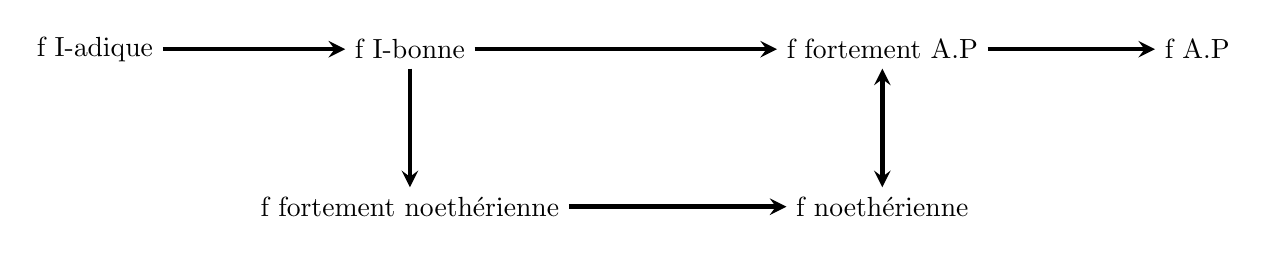
\begin{tikzpicture}
		% Création des nœuds
		\node (A) at (0,0) {f I-adique};
		\node (B) at (4,0) {f I-bonne};
		\node (C) at (4,-2) {f fortement noethérienne};
		\node (D) at (10,-2) {f noethérienne};
		\node (E) at (14,0) {f A.P};
		\node (F) at (10,0) {f fortement A.P};
		
		% Dessin des flèches avec des modifications pour les rendre plus visibles
		\draw[->, ultra thick, >=stealth] (A) -- (B);
		\draw[->, ultra thick, >=stealth] (B) -- (C);
		\draw[->, ultra thick, >=stealth] (B) -- (F);
		\draw[->, ultra thick, >=stealth] (C) -- (D);
		\draw[->, ultra thick, >=stealth] (F) -- (E);
		\draw[<->, ultra thick, >=stealth] (F) -- (D);
	\end{tikzpicture}
\end{center}


\end{maremarque}


